
\chapter{Visualisation}
\label{chap:tscope}

\newcommand{\event}[1]{\code{#1}\xspace}
\newcommand{\metric}[1]{\textsc{#1}\xspace}
\newcommand{\metrictopic}[1]{\textbf{\textsc{#1}}\xspace}

\status{Not written yet}

The behaviour of parallel programs is even harder to understand
than the behaviour of sequential programs.
Parallel programs may suffer from
any of the performance problems afflicting sequential programs,
as well as from several problems unique to parallel systems.
Many of these problems are quite hard
(or even practically impossible)
to diagnose without help from specialised tools.
In this chapter we describe a proposal for a tool
for profiling the parallel execution of Mercury programs,
a proposal whose implementation we have already started.
This tool is an adaptation and extension of the \tscope profiler
that was first built to help programmers visualise
the execution of parallel Haskell programs.

The structure of this chapter is as follows.
Section~\ref{sec:tscope_intro} describes three different groups of people,
Mercury programmers, runtime system implementors and automatic parallelism
researchers.
For each group we describe how a visual profiler based on \tscope would
benefit them.
Section~\ref{sec:tscope_background} gives a description of the \tscope tool,
how it is used in Haskell,
and how we can use it for Mercury without any modifications.
Section~\ref{sec:tscope_newevents}
describes how we modify and extended the \tscope system
to collect the kinds of data needed to more completely describe
the parallel execution of Mercury programs,
while Section~\ref{sec:tscope_analysis} describes how
one can analyse that data to yield insights
that can be useful to our three audiences:
application programmers,
runtime system implementors,
and the implementors of auto-parallelisation tools.
Section~\ref{sec:tscope_example} shows some examples of our work so far.
Finally, Section~\ref{sec:tscope_conc}
concludes with a discussion of related work.

\section{Introduction}
\label{sec:tscope_intro}

When programmers need to improve the performance of their program,
they must first understand it.
The standard way to do this is to use a profiler.
Profilers record performance data from executions of the program,
and give this data to programmers
to help them understand how their program behaves.
This enhanced understanding then makes it easier
for programmers to speed up the program.

Profilers are needed because the actual behaviour of a program
often differs from the behaviour assumed by the programmer.
This is true even for sequential programs.
For parallel programs,
the gulf between human expectations and machine realities
is usually even wider.
This is because every cause of unexpected behaviour
for sequential programs
is present in parallel programs as well,
while parallel programs also have several causes of their own.
% When writing software that uses parallelism,
% understanding how the program runs is more difficult.
% Parallelism may be used in different parts of the program,
% causing some parts to speed up while other parts remain sequential.

Consider a program containing a loop with many iterations
in which the iterations do not depend on one another
and can thus be done in parallel.
% is an independent parallel task.
Actually executing every iteration in parallel
may generate an overwhelming number of parallel tasks.
It may be that the average amount of computation done by one of these tasks
is less than the amount of work it takes to spawn one of them off.
In that case, executing all the iterations in parallel
will increase overheads to the point of actually slowing the program down,
perhaps quite substantially.
The usual way to correct this is to use granularity control
to make each spawned-off task execute
not one but several iterations of the loop,
thus making fewer but larger parallel tasks.
However, if this is done too aggressively,
performance may once again suffer.
For example,
there may be fewer tasks created than the computer has processors,
causing some processors to be idle when they could be used.
More commonly, the iterations of the loop and thus the tasks
may each need a different amount of CPU time.
If there are eight processors and eight unevenly sized tasks,
then some processors will finish their work early,
and be idle while waiting for the others.

All these problems can arise in programs with independent parallelism:
programs in which parallel tasks do not need to communicate.
Communication between tasks makes this situation even more complicated,
especially when a task may block waiting for information from another task.
A task that blocks may in turn further delay
other tasks that depend on data \emph{it} produces.
Chains of tasks that produce and consume values from one another are common,
Programmers need tools to help them
identify and understand performance problems,
whether they result from such dependencies or other causes.

Profiling tools that can help application programmers
can also be very useful for the implementors of runtime systems.
While optimising Mercury's parallel runtime system (Chapter~\ref{chap:rts}),
we have needed to measure the costs of certain operations
and the frequency of certain behaviours.
Some examples are:
when a piece of work is made available,
how quickly can a sleeping worker-thread respond to this request?
When a task is made runnable after being blocked,
how often will it be executed on the same CPU that was previously executing it,
so that its cache has a chance to be warm?
Such information from profiles of typical parallel programs
can be used to improve the runtime system,
which can help improve the performance of \emph{all} parallel programs.

A third category of people who can use profiling tools for parallel programs
are researchers working on automatic parallelisation tools
(Chapter~\ref{chap:overlap}).
Doing a good job of automatically parallelising a program
requires a cost-benefit analysis for each parallelism opportunity,
which requires estimates of both the cost and the benefit of each opportunity.
Profiling tools can help researchers calibrate
the algorithms they use to generate estimates of both costs and benefits.
We did not use the work in this chapter to help us with these problems in
Chapter~\ref{chap:overlap},
so using \tscope to tune the work of Chapter~\ref{chap:overlap} represents
some potential further work.
% For example, if it is more expensive to spawn off a computation
% than it is to execute it locally, we prefer to execute it locally.
% To answer this we need to know how expensive
% it is to spawn off the computation as a new task.
% We want to use profiling data from the parallel runtime to anwser this.

As researchers working on the parallel implementation of Mercury,
including automatic parallelism,
we fall into all three of the above categories.
We have long needed a tool
to help us understand the behaviour of parallel Mercury programs,
of the parallel Mercury runtime system
and of our auto-parallelisation tool (Chapter~\ref{chap:overlap}),
but the cost of building such a tool seemed daunting.
We therefore looked around for alternative approaches.
The one we selected was to adapt to Mercury
an existing profiler for another parallel system.

The profiler we chose was \tscope \citep{threadscope},
a profiler built by the team behind the Glasgow Haskell Compiler (GHC)
for their parallel implementation of Haskell.
We chose \tscope because
the runtime system it was designed to record information from
has substantial similarities to the Mercury runtime system,
because \tscope was \emph{designed} to be extensible,
and, like many visualisation tools, it is extremely useful
for finding subtle issues that cause significant problems.

% This paper presents the adaption of \tscope \citep{threadscope}
% --- a tool for profiling the parallel execution of Haskell programs
% --- to Mercury \citep{jlp} --- a pure logic programming language.
% We will use the above three types of users to determine the usefulness of our
% work.

\section{Existing \tscope events}
\label{sec:tscope_background}

\tscope was originally built
to help programmers visualise the parallel execution of Haskell programs
compiled with the dominant implementation of Haskell,
the Glasgow Haskell Compiler (GHC).
The idea is that during the execution of a parallel Haskell program,
the Haskell runtime system writes time-stamped reports
about significant events to a log file.
The \tscope tool later reads this log file,
and shows the user graphically what each CPU was doing over time.
The diagrams it displays reveal to the programmer
the places where the program is getting the expected amount of parallelism,
as well as the places where it is not.

We were able to adapt the \tscope system to Mercury for two main reasons.
The first is that the parallel implementations of Haskell and Mercury
in GHC and mmc (the Melbourne Mercury Compiler)
are quite similar in several important respects,
even though they use different terms for
(slightly different implementations of) the same concepts.
For example, what Mercury calls an engine GHC calls a \emph{capability},
and what Mercury calls a context GHC calls a \emph{thread}.
(Except where noted,
we will continue to use Mercury terminology as we have done so far in the
dissertation.)
Mercury and GHC both use sparks,
although GHC's sparks do not need to be evaluated,
and may be garbage collected.
The second reason
that we were able to adapt \tscope to Mercury is that
the \tscope log file format was designed to be extensible.
Each log file starts with a description
of each kind of event that may occur in it.
This description includes three fields:
\begin{itemize}
\item the event's id
\item a string that describes the event to users and implementors,
\item and the total size of the event,
which may be variable.
\end{itemize}
The fields within the event and their sizes and meanings are established by
convention.
This means that when the event has a variable size,
only one of the fields may have a variable size,
unless self-describing fields or extra fields that specify the sizes of
other fields are used.
This description is precise enough that tools
can skip events that they do not understand,
and process the rest.

Mercury is able to make use of a number of event types already supported by
\tscope and GHC,
and in other cases we are able to add support for Mercury-specific event
types to \tscope.
Here we introduce the events in the first category;
the next section describes those in the second category.
Events of all types have a 64bit timestamp
that records the time of their occurrence, measured in nanoseconds.
This unit illustrates the level of precision \tscope aims for,
although of course there is no guarantee
that the system clock is capable of achieving it.
Implementors are free to choose which clock they use to timestamp events.
The GHC implementors use the \code{gettimeofday(2)} system call,
and we use either \code{gettimeofday(2)} or the processors' time stamp
counters (TSCs).

Most events in the log file are associated with an engine.
To avoid having to include an engine id with every event in the log file,
the log file format
groups sequences of events that are all from the same engine into a block,
and writes out the engine id just once, in a block header pseudo-event.
Since tools reading the log file can trivially remember
the engine id in the last block header they have read,
this makes the current engine id
(the id of the engine in whose block an event appears)
an implicit parameter of most event types.

The event types supported by the original version of \tscope
that are relevant to our work are listed here.

\begin{description}

\item[STARTUP]
marks the beginning of the execution of the program,
and records the number of engines that the program will use.

\item[SHUTDOWN]
marks the end of the execution of the program.

\item[CREATE\_THREAD]
records the act of the current engine creating a context,
and gives the id of the context being created.
(What Mercury calls a context Haskell calls a thread;
the name of the event uses Haskell terminology.)
Context ids are allocated sequentially,
but the id cannot be omitted,
since the runtime system may reuse the storage of a context
after the termination of the computation that has previously used it,
and therefore by specifying the id we can determine when a thread is reused.

\item[RUN\_THREAD]
records the scheduling event
of the current engine switching to execute a context,
and gives the id of the context being switched to.

\item[STOP\_THREAD]
records the scheduling event
of the current engine switching away from executing a context.
Gives the id of the context being switched from,
as well as the reason for the switch.
The possible reasons include:
(a) the heap is full, and so the engine must invoke the garbage collector;
(b) the context has blocked, and
(c) the context has finished.
GHC uses many more reason values, but these are the only reasons that
are applicable to our work.
The context id could be derived implicitly,
but the convention that was established by the GHC developers requires us to
provide it.

\item[THREAD\_RUNNABLE]
records that the current engine has made a blocked context runnable,
and gives the id of the newly-runnable context.

\item[RUN\_SPARK]
records that the current engine is starting to run a spark
that it retrieved from its own local spark queue.
Gives the id of the context that will execute the spark,
although, like \event{STOP\_THREAD}, this can be inferred by context.
However the inference required is slightly different between GHC and Mercury.
% \zoltan{It can be inferred from the context id of the next
% CREATE\_SPARK\_THREAD event in Mercury,
% is this true in Haskell as well?}

\item[STEAL\_SPARK]
records that the current engine will run a spark
that it stole from the spark queue of another engine.
Gives the id of the context that will execute the spark,
although again, this can be inferred by context.
% \zoltan{It can be inferred from the context id of the next
% CREATE\_SPARK\_THREAD event in Mercury,
% is this true in Haskell as well?}
Also gives the id of the engine that the spark was stolen from.
% This should really be called STOLE_SPARK.

\item[CREATE\_SPARK\_THREAD]
is slightly different in GHC and Mercury.
In GHC this records the creation of a worker context that runs a special
routine that processes sparks in a loop;
this can be thought of as a worker context for executing sparks.
In Mercury this event is recorded when an engine wishes to execute a particular
spark and needs a new context to do it;
the context may be used to execute subsequent sparks.
The event gives the id of the context.
The context may be an existing context that is reused,
but the event does not say whether the context is new or reused.
In most cases, that information is simply not needed,
but if it is, it can be inferred from context.
% In both Mercury and Haskell,
% the context will probably be used to execute other sparks
% once it finishes the current one.

\item[GC\_START]
is used when the current engine has initiated garbage collection;
control of the engine has been taken away from the mutator.
The garbage collection events in GHC are much more complex.
However, since Mercury uses the
Boehm-Demers-Weiser conservative garbage collector (Boehm GC)
\citep{boehm:1988:gc},
we have much less insight into the garbage collector's (GC) behaviour,
and thus fewer GC related events and simpler semantics.

\item[GC\_END]
indicates when garbage collection has finished on the current engine;
control of the engine has been returned to the mutator.
% \paul{I do not know the intended semantics of the GC events that Haskell uses}
% More information about how Mercury uses these events is in Section
% \ref{sec:gc_stats} below.

\end{description}

The longer a parallel program being profiled runs,
the more events it will generate.
Long running programs can generate enormous log files.
To keep the sizes of log files down as much as possible,
events include only the information they have to.
If some information about an event
can be inferred from information recorded for other events,
then the design principles of \tscope say
that information should be inferred at analysis time
rather than recorded at profiling runtime.
(The presence of context ids in \event{RUN\_SPARK} and \event{STEAL\_SPARK}
events is considered a mistake \citep{threadscope-summit},
since they are guaranteed to be the same as the id of the context already
running on that engine or
the context id in the following \event{CREATE\_SPARK\_THREAD} event,
but their removal is prevented by backwards compatibility concerns.)
In most cases, the required inference algorithm is quite simple.
For example, answering the question of whether the context
mentioned by a \event{CREATE\_SPARK\_THREAD} event is new or reused
merely requires searching the part of the log up to that event
looking for mentions of the same context id.
We have already seen how the engine id parameter
missing from most of the above events
can be deduced from block headers.

\section{New events}
\label{sec:tscope_newevents}

In order to support the profiling of parallel Mercury programs,
we had to add new arguments to two of the existing \tscope events.
Originally, the \event{RUN\_SPARK} and \event{STEAL\_SPARK} events
did \emph{not} specify the identity of the spark being run or stolen.
This is not a problem for the Haskell version of \tscope,
since the implementors did not care about sparks' identities
\citep{threadscope-summit}.
However, we do, since sparks correspond to conjuncts in parallel conjunctions,
and we want to give to the user not just general information
about the behaviour of the program as a whole,
but also about the behaviour of individual parallel conjunctions,
and of the conjuncts in them.
We have therefore added an id that uniquely identifies each spark
as an additional argument of the \event{RUN\_SPARK} and \event{STEAL\_SPARK}
events.
Note that \event{CREATE\_SPARK\_THREAD} does not need a spark id,
since the only two ways it can get the spark it converts into a context
is by getting it from its own queue or from the queue of another engine.
A \event{CREATE\_SPARK\_THREAD} event will therefore always be preceded
by either a \event{RUN\_SPARK} event or a \event{STEAL\_SPARK} event,
and the id of the spark in that event
will be the id of the spark being converted.

% In Haskell, their identities can always be inferred
% by modelling the spark queues of all the capabilities (engines) in the system.

We have extended the set of \tscope event types
to include several new types of events.
Most of these record information about constructs that do not exist in Haskell:
parallel conjunctions, conjuncts in those conjunctions, and futures.
Some provide information about the behaviour of Mercury engines
that \tscope for Haskell does not need,
either because that information is of no interest,
or because the information is of interest
but it can be deduced from other events.
Even though the Haskell and Mercury runtime systems
generate many of the same events,
the stream of these common events they generate
do not necessarily obey the same invariants.

However, most of the work we have done towards adapting \tscope to Mercury
has been in the modification of the parallel Mercury runtime system
to generate all of the existing, modified and new events when called for.

In the rest of this section,
we report on the event types we have added to \tscope.
In the next section, Section~\ref{sec:tscope_analysis},
we will show how the old and new events can be used together
to infer interesting and useful information
about the behaviour of parallel Mercury programs.

\begin{description}

\item[STRING] records an association between a text string and an integer so
that a string occurring many times within a log file can be
replaced with an integer.
Making the log files shorter and therefore not flushing them to disk
as often.

\item[START\_PAR\_CONJUNCTION] records the fact that
the current engine is about to start executing a parallel conjunction.
It identifies the parallel conjunction in two different ways.
The static id identifies
the location of the conjunction in the source code of the program.
The dynamic id is the address of the barrier structure
that all the conjuncts in the conjunction will synchronise on when they finish.
Note that barrier structures' storage may be reused for other objects,
including other barriers, by later code,
so these dynamic ids are not unique across time,
but they \emph{do} uniquely identify a parallel conjunction
at any given moment in time.
See the end of this section for a discussion of why we chose this design.

\item[END\_PAR\_CONJUNCTION]
records the end of a parallel conjunction.
It gives the dynamic id of the finishing conjunction.
Its static id can be looked up in the matching
\event{START\_PAR\_CONJUNCTION}
event.

\item[CREATE\_SPARK] records the creation of a spark
for a parallel conjunct by the current engine.
% \paul{XXX We call this SPARKING in the source code but should not}
It gives the id of the spark itself,
and the dynamic id of the parallel conjunction containing the conjunct.
To keep the log file small,
it does \emph{not} give the position of the conjunct in the conjunction.
However, since in every parallel conjunction
the spark for conjunct $n+1$
will be created by the context executing conjunct $n$,
and unless $n=1$, that context will itself have been created
from the spark for conjunct $n$.
(The first conjunct of a parallel conjunction is always executed directly,
without ever being represented by a spark.)
This means that the sparks for the non-first conjuncts
will always be created in order,
which makes it quite easy to determine which spark represents which conjunct.

The id of a spark is an integer consisting of two parts:
% spark IDs are 32 bits wide, the 8 most significant bits are the engine ID,
the first part is the id of the engine that created the spark,
and the second is an engine-specific sequence number,
so that in successive sparks created by the same engine,
the second part will be 1, 2, 3 etc.
This design allows the runtime system
to allocate globally unique spark ids without synchronisation.

\item[END\_PAR\_CONJUNCT]
records that the current engine
has finished the execution of a conjunct in a parallel conjunction.
It also gives the dynamic id of the parallel conjunction.
Note that there is no \event{START\_PAR\_CONJUNCT} event
to mark the start of execution of any conjunct.
For the first conjunct, its execution will start
as soon as the engine has finished recording the
\event{START\_PAR\_CONJUNCTION} event.
The first thing the conjunct will do is create a spark
representing the second and later conjuncts
(which above we informally referred to as the spark for the second conjunct).
The \event{CREATE\_SPARK} event records the id of the spark,
then, either the \event{RUN\_SPARK} event or \event{STEAL\_SPARK} event records
which engine and context executes the spark.
If the engine does not yet have a context a \event{CREATE\_SPARK\_THREAD}
event is posted that identifies the newly created context.
\event{RUN\_THREAD} and \event{STOP\_THREAD} events
also tell us when that context is executing, and on which engine.
The first thing the second conjunct does is spawn off a spark
representing the third and later conjuncts.
By following these links,
a single forward traversal of the log file can find out,
for each engine, which conjunct of which dynamic parallel conjunction
it is running at any given time
(if in fact it is running any:
an engine can be idle,
or it may be running code that is outside of any parallel conjunction).
When an engine records an \event{END\_PAR\_CONJUNCT} event,
it can only be for the conjunct it is currently executing.

\item[FUTURE\_CREATE] records the creation of a future by the current
engine.
It gives the name of the variable the future is for,
as well as the dynamic id of the future.
It does not give the dynamic id of the parallel conjunction
whose conjuncts the future is intended to synchronise,
but that can be determined quite easily:
just scan forward for the next \event{START\_PAR\_CONJUNCTION}
event.
The reason why this inference works is that
the code that creates futures
is only ever put into programs by the Mercury compiler,
which never puts that code anywhere
except just before the start of a parallel conjunction.
If a parallel conjunction uses $n$ futures,
then every one of its \event{START\_PAR\_CONJUNCTION} events
will be preceded by $n$ \event{FUTURE\_CREATE} events,
one for each future.

The dynamic id of the future is its address in memory.
This has the same reuse caveat
as the dynamic ids of parallel conjunctions.

\item[FUTURE\_SIGNAL] records that code running on the current engine
has signalled the availability
of the value of the variable protected by a given future.
The event provides the id of the future.
If another conjunct is already waiting for the value stored in this future,
then its context is now unblocked.

\item[FUTURE\_WAIT\_NO\_SUSPEND] records that the current engine
retrieved the value of the future without blocking.
Gives the id of the future.
The future's value was already available
when the engine tried to wait for the value of the future,
so the context running on the current engine was not blocked.

\item[FUTURE\_WAIT\_SUSPEND] records that the current engine
tried to retrieve the value of a future, but was blocked.
Gives the id of the future.
Since the future's value was not already available,
the current context has been be suspended until it is.

\end{description}

We have added a group of four event types
that record the actions of engines
that cannot continue to work on what they were working before,
either because the conjunct they were executing finished,
or because it suspended.

\begin{description}

\item[TRY\_GET\_RUNNABLE\_CONTEXT] records when the engine is checking the
global run queue for a context to execute.

\item[TRY\_GET\_LOCAL\_SPARK] records that this engine is attempting to get
a spark from its own deque.

\item[TRY\_STEAL\_SPARK] records that this engine is attempting to steal a
spark from another engine.

\item[ENGINE\_WILL\_SLEEP] records that the engine is about to sleep.
The next event from this engine will be from when it is next awake.

\end{description}

\noindent
The idea is that an idle engine can look for work in three different places:
(a) the global runnable context queue,
(b) its own local spark queue, and
(c) another engine's spark queue.
An idle engine will try these in some order,
the actual order depending on the scheduling algorithm.
The engine will post the try event for a queue
before it actually looks for work in that queue.
If one of the tests is successful, the engine will post
a \event{START\_THREAD} event, a \event{RUN\_SPARK} event or a
\event{STEAL\_SPARK} event respectively.
If one of the tests fails, the engine will go on the next.
If it does not find work in any of the queues,
it will go to sleep after posing the \event{ENGINE\_WILL\_SLEEP} event.

This design uses two events to record
the successful search for work in a queue:
\event{TRY\_GET\_RUNNABLE\_CONTEXT} and \event{START\_THREAD},
\event{TRY\_GET\_LOCAL\_SPARK} and \event{RUN\_SPARK},
or \event{TRY\_STEAL\_SPARK} and \event{STEAL\_SPARK}.
This may seem wasteful compared to using one event,
but this design enables us to measure several interesting things:

\begin{itemize}
\item
how quickly a sleeping engine can wake up and try to find work
when work is made available by a \event{CREATE\_SPARK} and or
\event{CONTEXT\_RUNNABLE} event;
% This can remove the space between items, as well as above and below
% the environment, I like the look of -0.5
% \vspace{-1\baselineskip}
\item
how often an engine is successful at finding work;
% \vspace{-1\baselineskip}
\item
when it is successful,
how long it takes an engine to find work and begin its execution;
% \vspace{-1\baselineskip}
\item
when it is unsuccessful,
how long it takes to try to find work from other sources,
fail, and then to go to sleep.
\end{itemize}
%\vspace{-2mm}

% I have removed the idle and working events.
% I spoke with Simon Marlow about this, I cannot construct a sound
% argument why I need them, and in all cases the state of an engine
% can be inferred by other events.  Although this inference feels
% dirty/clumsy it is the correct option since it keeps the log file
% shorter.
% The problem now is that Haskell and Mercury both behave differently,
% and therefore may have different rules of inference.

As we mentioned above,
using the address of the barrier structure
as the dynamic id of the parallel conjunction whose end the barrier represents
and using the address of the future structure
as the dynamic id of the future
are both design choices.
The obvious alternative would be to give them both sequence numbers
using either global or engine-specific counters.
However, this would require
adding a field to both structures to hold the id, which costs memory, and
filling in the field, which costs time.
Both these costs would be incurred by the program execution
whose performance we are trying to measure,
interfering with the measurement itself.
While such interference cannot be avoided
(writing events out to the log file also takes time),
we nevertheless want to minimise it if at all possible.
In this case, it is possible:
the addresses of the structures are trivially available,
and require no extra time or space during the profiled run.

The tradeoff is that if an analysis requires globally unique dynamic ids
for parallel conjunctions or for futures,
and most analyses do,
then it needs to ensure that a pre-pass has been run over the log file.
This pre-pass would maintain a map from future ids
to a pair containing an active/inactive flag, and a replacement id,
and another map from dynamic conjunction ids
to a tuple containing an active/inactive flag, a replacement id,
and a list of future ids.
When the pre-pass sees a dynamic conjunction id or future id in an event,
it looks it up in the relevant table.
If the flag says the id is active,
it replaces the id with the replacement.
If the flag says the id is inactive,
it gets a new replacement id (e.g.\ by incrementing a global counter),
and sets the flag to active.
If the event is a \event{FUTURE\_CREATE} event,
the pre-pass adds the future's original id to a list.
If the event is a \event{START\_PAR\_CONJUNCTION} event,
it copies this list to the conjunction's entry, and then clears the list.
If the event is an \event{END\_PAR\_CONJUNCTION} event,
which ends the lifetime not only of the parallel conjunction
but also of all futures created for that conjunction,
the pre-pass sets to inactive
that flags of both the conjunction itself
and the futures listed in its entry.

This algorithm consistently renames apart
the different instances of the same id,
replacing them with globally unique values.
Its complexity can be close to linear, provided
the maps are implemented using a suitable data structure, such as a hash table.
This transformation does not even need an extra traversal of the log file data.
The \tscope tool must traverse the log file anyway
when it gets ready to display its contents,
and this transformation can be done
as part of that traversal.
The extra cost is therefore quite small.


\section{Deriving metrics from events}
\label{sec:tscope_analysis}

\tscope is primarily used to visualise the execution of parallel programs.
However, we can also use it, along with our new events,
to calculate and to present to the user
a number of different metrics about the execution of parallel Mercury programs.
The GHC developers have independently\footnote{
    The GHC developers added the alternative views to \tscope after we
    published the paper on which this chapter is based
    \citep{bone:2011:tscope}.}
recognised this need,
and have created alternative views within the \tscope GUI to present textual
information such as reports of these metrics.
In our rudimentary prototype of how these metrics could be calculated we
used a command line driven console interface.
(Some parts of \tscope are implemented as a library,
allowing the development of different independent tools.)
% \zoltan{needs discussion about how metrics are presented to users}
% \zoltan{needs discussion about audiences}
Some of the metrics are of interest
only to application programmers,
or only to runtime system implementors,
or only to auto-parallelisation tool implementors,
but several are useful to two or even all three of those groups.
Also, metrics can be organised by their \emph{subject},
whether that is:
\begin{itemize}
    \item the whole program,

    \item an engine,

    \item a parallel conjunction,

    \item a parallel conjunct,

    \item a future.
\end{itemize}
We discuss our proposed metrics in that order;
we then discuss how we intend to present them to users.

% Such as how much overlap we are \emph{really} getting,
% and how efficient the RTS is and how this can drive settings in our
% automatic parallelisation analysis.
%
% Discuss granularity and parallel slackness, show how we can measure these.

\subsection{Whole program metrics}

% \emph{PARCONJ\_CONTEXT\_SELF:
% The number of contexts that are actually used
% by a given parallel conjunction.}
% This measurement is computed similarly to PARCONJ\_RUNNABLE\_SELF,
% but it does not count the part of a conjunct's lifetime
% that it spends as a spark;
% it counts only the part that it spends as a context.
% The difference is important,
% because contexts occupy substantial amounts of memory,
% while sparks do not.

% For optimum memory efficiency,
% the ratio between the time-weighted averages of
% PARCONJ\_CONTEXT\_SELF and PARCONJ\_RUNNABLE\_SELF
% should be as low as possible for all parallel conjuncts.

\metrictopic{CPUs over time}
is the number of CPUs being used by the program at any given time.
It is trivial to scan all the events in the trace,
keeping track of the number of engines currently being used,
each of which corresponds to a CPU.
The resulting curve tells programmers
which parts of their program's execution is already sufficiently parallelised,
which parts are parallelised but not yet enough to use all available CPUs,
and which parts still have no parallelism at all.
They can then focus their efforts on the latter.
The visualisation of this curve is already implemented in \tscope
\citep{threadscope}.

% \label{sec:gc_stats}
\metrictopic{GC stats} is the number of garbage collections,
and the average, minimum, maximum and variance
of the elapsed time taken by each collection.
%Mercury uses the Boehm-Demers-Weiser garbage collector \citep{boehm:1988:gc}.
Boehm GC supports parallel marking using GC-specific helper threads
rather than the OS threads that run Mercury engines.
Therefore, even when parallel marking is used,
we can only calculate the elapsed time used by garbage collection,
and not the \emph{CPU time} used by garbage collection.
The elapsed time of each garbage collection
is the interval between pairs of \event{GC\_START} and \event{GC\_END}
events.

\metrictopic{Mutator vs GC time}
is the fraction of the program's runtime used by the garbage collector.
We calculate this by summing the times
between pairs of \event{GC\_START} and \event{GC\_END} events,
and dividing the result by the program's total runtime.
(Both sides of the division refer to elapsed time, not CPU time.)
Due to Amdahl's law \citep{amdahl:1967:law},
% Explain amdahl's law since the paper dosn't describe the usual
% interpretation.
the fraction of time spent in garbage collection limits the best possible
speedup we can get for the program as a whole by parallelising the mutator.
For example, if the program spends one third of its time doing GC
(which unfortunately actually happens for some parallel programs),
then no parallelisation of the program can yield a speedup of more than three,
\emph{regardless} of the number of CPUs available.

\metrictopic{Nanosecs per call}
is the average number of nanoseconds between successive procedure calls.
The Mercury deep profiler (for sequential programs) \citep{conway:2001:mercury-deep}
(Section~\ref{sec:backgnd_deep}),
which has nothing to do with \tscope,
measures time in call sequence counts (CSCs);
the call sequence counter is incremented at every procedure call.
It does this because there is no portable, or even semi-portable way
to access any real-time clocks that may exist on the machine,
and even the non-portable method on x86 machines (the RDTSC instruction)
is too expensive for it.
(The Mercury sequential profiler needs to look up the time at every call,
which in typical programs will happen every couple of dozen instructions or so.
The Mercury runtime support for \tscope needs to look up the time only at
each event,
which occur \emph{much} less frequently.)
% RDTSC still has some overhead:
% a) It is a sequencing operation for the CPU.
% b) It requires some arithmetic and maybe a function call, I do not
%    know if we can afford that.

The final value of the call sequence counter
at the end of a sequential execution of a program
gives its length in CSCs; say $n$ CSCs.
When a parallelised version of the same program is executed on the same data
under \tscope,
we can compute the total amount of \emph{user time}
taken by the program on all CPUs; say $m$ nanoseconds.
The ratio $n/m$ gives the average number of nanoseconds
in the parallel execution of the program
per CSC in its sequential execution.
% \paul{I am having trouble parsing the above sentence, I ave tried to
% read it 3 times now, I do not know what you're trying to say}
% \zoltan{is the new phrasing clear?}
% Clearer, but not great, I get stuck at ``in its sequential execution''
% but now I know what you mean and this phrase is somewhat implicit.
This is useful information,
because our automatic parallelisation system
uses CSCs, as measured by the Mercury sequential profiler,
as its unit of measurement of the execution time
of both program components and system overheads.
Using this scale, we can convert predictions about time made by the tool
from being expressed in CSCs to being expressed in nanoseconds,
which is an essential first step in comparing them to reality.

\metrictopic{Contexts allocated} is the number of contexts allocated at any given
time;
it includes contexts that are running, runnable and blocked.

\metrictopic{Contexts runnable} is the number of contexts that are on the global
context run queue at any given time.

% number of sparks plus runnable but not running contexts at any given time


\subsection{Per engine metrics}

\metrictopic{Sparks available}
is the number of sparks available for execution at any given time.
Since the time of publishing \citet{bone:2011:tscope} the GHC developers
added similar metrics to \tscope.
Their metrics are more complicated as their spark implementation is more
complicated.
Their implementation introduces a new event that provides summary data just
for this purpose;
by comparison our spark events provide more detail as we know more accurately
when each spark event occurred.
We wish to measure the number of sparks available on each Mercury engine's
deque at any given time.
This can be done by maintaining a counter for each engine,
incrementing it each time that engine uses the \event{CREATE\_SPARK} event,
and decrementing it whenever the engine uses a \event{RUN\_SPARK} event or
another engine uses a \event{STEAL\_SPARK} event for a spark on this
engine's deque.


\subsection{Conjunction specific metrics}

\metrictopic{Parconj time} is the time taken by a given parallel conjunction.
For each dynamic parallel conjunction id that occurs in the trace,
it is easy to compute the difference between
the times at which that parallel conjunction starts and ends,
and it is just as trivial to associate these time intervals
with the conjunction's static id.
From this, we can compute,
for each parallel conjunction in the program that was actually executed,
both the average time its execution took,
and the variance in that time.
This information can then be compared,
either by programmers or by automatic tools,
with the sequential execution time of that conjunction recorded by
Mercury's deep profiler,
to see whether executing the conjunction in parallel was a good idea or not,
\emph{provided} that the two measurements are done in the same units.
At the moment, they are not, but as we discussed above,
CSCs can be converted to nanoseconds using the \metric{Nanosecs per call}
metric.

\metrictopic{Parconj runnable self}
is the number of CPUs that can be used by a given parallel conjunction.
For each dynamic parallel conjunction id that occurs in the trace,
we can divide the time between its start and end events into blocks,
with the blocks bounded by
the \event{CREATE\_SPARK\_THREAD} and \event{STOP\_THREAD} events for its
conjuncts,
and the \event{FUTURE\_WAIT\_SUSPEND} and \event{FUTURE\_SIGNAL} events
of the futures used by those conjuncts.
We can then compute, for each of these blocks,
the number of runnable tasks that these conjuncts represent.
From this we can compute the history of the number
of runnable tasks made available by this dynamic conjunction.
We can derive the maximum and the time-weighted average of this number,
and we can summarise those
across all dynamic instances of a given static conjunction.

Consider a conjunction with $n$ conjuncts.
If it has a maximum number of runnable tasks
significantly less than $n$,
this is a sign that the parallelism the programmer aimed for
could not be achieved.
If instead the average but not the maximum number of runnable tasks
is significantly less than $n$,
this suggests that the parallelism the programmer aimed for was achieved,
but only briefly.
The number of runnable tasks can drop due to
either a wait operation that suspends or the completion of a conjunct.
Both dependencies among conjuncts
and differences in the execution times of the conjuncts
limit the amount of parallelism available in the conjunction.
The impact of the individual drops on the time-weighted average
shows which effects are the most limiting in any given parallel conjunction.

\metrictopic{Parconj runnable self and descendants}
is the number of CPUs that can be used by a given parallel conjunction
and its descendants.
This metric is almost the same as \metric{Parconj runnable self},
but it operates
not just on a given dynamic parallel conjunction,
but also on the parallel conjunctions
spawned by the call-trees of its conjuncts as well.
It takes their events into account when it divides time into blocks,
and it counts the number of runnable tasks they represent.

The two metrics,
\metric{Parconj runnable self} and
\metric{Parconj runnable self and descendants},
can be used together to see whether
the amount of parallelism that can be exploited
by the two parallel conjunctions together is substantially greater than
the amount of parallelism that can be exploited
by just the outer parallel conjunction alone.
If it is, then executing the inner conjunction in parallel is a good idea;
if it is not, then it is a bad idea.

If the outer and inner conjunction in the dynamic execution
come from different places in the source code,
then acting on such conclusions is relatively straightforward.
If they represent different invocations of the same conjunction in the program,
which can happen if one of the conjuncts contains a recursive call,
then acting on such conclusions will typically require
the application of some form of runtime granularity control.

% \paul{The number of parallel conjunctions in this case is as deep as
% the recursion, not just two.
% Can you explain how considering the first two levels of the recursion
% bares on all the levels of recursion?
% Or is this a case where a parallel conjunction is nested within
% another and no code within either conjunction is recursive?  Thanks}

\metrictopic{Parconj running self}
is the number of CPUs that are actually used by a given parallel conjunction.
This metric is computed similarly to \metric{Parconj runnable self},
but it does not count a runnable conjunct until gets to use a CPU,
and stops counting a conjunct when it stops using the CPU
(when it blocks on a future, and when it finishes).
% \zoltan{Does the CPU ever get taken away from a conjunct?}
% \paul{Only when it blocks on a future, finishes a conjunct or calls
% \code{sched.yield}}

Obviously, \metric{Parconj running self} can never exceed
\metric{Parconj runnable self}
for any parallel conjunction at any given point of time.
However, one important difference between the two metrics
is that \metric{Parconj running self} can never exceed
the number of CPUs on the system either.
If the maximum value of \metric{Parconj runnable self} for a parallel
conjunction
does not exceed the number of CPUs,
then its \metric{Parconj running self} metric
can have the same value as its \metric{Parconj runnable self} metric,
barring competition for CPUs by other parallel conjunctions (see later)
or by the garbage collector.

On the other hand, some conjunctions
do generate more runnable tasks than there are CPUs.
In such cases, we want the extra parallelism
that the system hardware cannot accommodate
in the period of peak demand for the CPU
to ``fill in'' later valleys,
periods of time when the conjunction demands
less than the available number of CPUs.
This will happen only to the extent that
such valleys do not occur after a barrier at the end of the period of time
where there is an abundance of parallelism,
or that the delayed execution of tasks that lost the competition for the CPU
does not lead to further delays in later conjuncts
through variable dependencies.

The best way to measure this effect
is to visually compare the \metric{Parconj running self} curves for the
conjunction taken from two different systems,
e.g.\ one with four CPUs and one with eight.
However, given measurements taken from e.g.\ a four CPU system,
it should also be possible to predict with \emph{some} certainty
what the curve would look like on an eight CPU system,
by using the times and dependencies recorded in the four-CPU trace
to simulate how the scheduler would handle the conjunction
on an eight CPU machine.
Unfortunately, the simulation cannot be exact
unless it correctly accounts for \emph{everything},
including cache effects and the effects on the GC system.

The most obvious use of the \metric{Parconj running self} curve of a
conjunction is to tell programmers whether and to what extent
that parallel conjunction can exploit the available CPUs.

\metrictopic{Parconj running self and descendants}
is the number of CPUs that are actually used by a given parallel conjunction
and its descendants.
This metric has the same relationship to
\metric{Parconj running self}
as \metric{Parconj runnable self and descendants} has to
\metric{Parconj runnable self}.
Its main use is similar to the main use of \metric{Parconj running self}:
to tell programmers whether and to what extent
that parallel conjunction and its descendants can exploit the available CPUs.
This is important because a conjunction and its descendants
may have enough parallelism
even if the top-level conjunction by itself does not,
and in such cases the programmer can stop looking for more parallelism,
at least in that part of the program's execution timeline.

\metrictopic{Parconj available CPUs}
is the number of CPUs available to a given parallel conjunction.
Scanning through the entire trace,
we can compute and record the number of CPUs being used
at any given time during the execution of the program.
For any given parallel conjunction,
we can also compute \metric{Parconj running self and descendants},
the number of CPUs used by that conjunction and its descendants.
By taking the difference between the curves of those two numbers,
we can compute the curve of the number of CPUs
that execute some task \emph{outside} that conjunction,
Subtracting that difference curve
from the constant number of the available CPUs
gives the number of CPUs available for use by this conjunction.

This number's maximum, time-weighted average
and the shape of the curve of its value over time,
averaged over the different dynamic occurrences
of a given static parallel conjunction,
tell programmers the level of parallelism they should aim for.
Generating parallelism in a conjunction
that consistently exceeds the number of CPUs available for that conjunction
is more likely to lead to slowdowns from overheads
than to speedups from parallelism.

\metrictopic{Parconj continue on before}
is the frequency, for any given parallel conjunction,
that the code after the conjunction
will continue executing on the same CPU
as the code before the conjunction.
If the parallel conjunction as a whole took only a small amount of time,
then CPUs other than the original CPU will still have relatively cold caches,
even if they ran some part of the parallel conjunction.
We want to keep using the warm cache of the original CPU.
The better the scheduling strategy is at ensuring this,
the more effectively the system as a whole will exploit the cache system,
and the better overall system performance will be.

\metrictopic{Parconj continue on last}
is the frequency, for any given parallel conjunction,
that the code after the conjunction
will continue executing on the same CPU
as the last conjunct to finish.
If the parallel conjunction as a whole took a large amount of time,
then how warm the cache of a CPU will be
for the code after the conjunction
depends on how recently that CPU executed
either a conjunct of this conjunction or the code before the conjunction.
Obviously, all the conjuncts execute after the code before the conjunction,
so if the conjunction takes long enough for most of the data accessed
before the conjunction to
% \paul{Cached data does not become cold, a cache becomes cold after
% useful data has been removed}.
% become cold and therefore
be evicted from the cache,
then only the CPUs executing the conjuncts will have useful data in
their caches.
% \paul{what race?}
% are in the race.
In the absence of specific information
about the code after the conjunct preferentially accessing data
that was also accessed (read or written) by specific conjuncts,
the best guess is that the CPU with the warmest cache
will be the one that last executed a conjunct of this conjunction.
The more often the scheduling strategy executes
the code after the conjunction on that CPU,
the more effectively the system as a whole will exploit the cache system,
and the better overall system performance will be.

\subsection{Conjunct specific metrics}

There are several simple times
whose maximums, minimums, averages and variances
can be computed for each static parallel conjunct.

\metrictopic{Conjunct time as spark}
is the time between the conjunct's creation
(which will be as a spark) and the start of its execution
(when the spark will be converted into a context).

\metrictopic{Conjunct time as context}
is the time between the start of the conjunct's execution and its end.

\metrictopic{Conjunct time blocked}
is the total amount of time
between the start of the conjunct's execution and its end
that the conjunct spends blocked waiting for a future.

% We also want a new metric,
% \item[CONJUNCT_TIME_BLOCKED_BARRIER] but discussing this means
% discussing right vs left recursion with Mercury's parallel runtime,
% which like to avoid for this paper.

\metrictopic{Conjunct time runnable}:
is the total amount of time
between the start of the conjunct's execution and its end
that the conjunct spends runnable but not running.

\metrictopic{Conjunct time running}
is the total amount of time
between the start of the conjunct's execution and its end
that the conjunct spends actually running on a CPU.

Since every context is always either running, runnable or blocked,
the last three numbers must sum up to the second
(in absolute terms and on average, not in e.g.\ maximum or variance).

Programmers may wish to look at conjuncts
that spend a large percentage of their time blocked
to see whether the dependencies that cause those blocks can be eliminated.

If such a dependency cannot be eliminated,
it may still be possible to improve
at least the memory impact of the conjunct
by converting some of the blocked time into spark time.
The scheduler should definitely prefer executing an existing runnable context
over taking a conjunct that is still a spark,
converting the spark into a context and running that context.
When there are no existing runnable contexts
and it must convert a spark into a context,
the scheduler should try to choose a spark whose consumed variables
(the variables it will wait for) are all currently available.
Of course, such a scheduling algorithm is not possible
without information about which variables conjuncts consume,
information that schedulers do not typically have access to,
but which it is easy to give them.

If all the sparks consume at least one variable
that is not currently available,
the scheduler should prefer to execute the one
whose consumed variables are the \emph{closest} to being available.
This requires knowledge of the expected behaviour of the program,
to wit, the expected running times of the conjuncts generating those variables.
In some cases, that information may nevertheless be available,
derived from measured previous runs of the program,
although of course it can only ever be an approximation.

Note also this is only one of several considerations
that an ideal scheduler should take into account.
For example, schedulers should also prefer to execute the conjunct
(whether it is a context or a spark)
that is currently next on the critical path to the end of the conjunction.
Knowledge of the critical path is also knowledge about the future,
and similarly must also be an approximation.
Ideally, the scheduler should take into account
all these different considerations before coming to a decision
based on balancing their relevance in the current situation.

% When it chooses between several existing runnable contexts,
% ideally it should choose one XXX

% If such a dependency cannot be eliminated,
% the programmer may still be able to improve
% at least the memory impact of the conjunct
% by converting some of the blocked time into spark time.
% The idea is that if a conjunct starts but then blocks waiting for some data,
% and does not generate any of its own data in the meantime,
% then if possible its start should be delayed
% until a time closer to when the data it needs will be available.
% This reduces the contribution made by the conjunct
% to the integral of the program's aggregate memory demand over time.
% Such as delay is often possible
% by merging two parallel conjuncts in a larger parallel conjunction into one.

% As an example, consider the three-way parallel conjunction
% p(In1, X, W) & q(In2, X, Y) & r(In3, Y, Z),
% where In1, In2 and In3 are available at the start of the conjunction,
% p generates X and W, q generates Y and r generates Z.
% If r needs Y very soon after the start of its execution,
% then it maybe preferable to change that conjunction into the two-way
% p(In1, X, W) & ( q(In2, X, Y), r(In3, Y, Z) ).
% By executing q and r in sequence instead of in parallel, ...
% XXX this example illustrates the wrong point

\metrictopic{Conjunct time after}
is the time, for each parallel conjunct,
between the end of its execution and the end of the conjunction as a whole.
It is easy to compute this for every dynamic conjunct,
and to summarise it as a minimum, maximum, average and variance
for any given static conjunct.
If the average \metric{Conjunct time after} metrics
for different conjuncts in a given parallel conjunction
are relatively stable (have low variance)
but differ substantially compared to the runtime of the conjunction as a whole,
then the speedup from the parallel execution of the conjunction
will be significantly limited by overheads.
% \paul{XXX: Amdahl or overhead?}
In such cases, the programmer may wish to take
two conjuncts that are now executed in parallel
and execute them in sequence.
Provided the combined conjunct is not the last-ending conjunct,
and provided that delaying the execution of one of the original conjuncts
does not unduly delay any other conjuncts that consume the data it generates,
the resulting small loss of parallelism
may be more than compensated for
by the reduction in parallelism overhead.
It is of course much harder
to select the two conjuncts to execute in sequence
if the times after for at least some of the conjuncts
are \emph{not} stable (i.e. they have high variance).

\metrictopic{Out of order frequency}:
given two parallel conjuncts $A$ and $B$,
with $A$ coming logically before $B$
either by being to the left of $B$ in some conjunction,
or by some ancestor of $A$ being to the left of an ancestor of $B$
in some conjunction,
how much time does the system spend with $B$ running
while $A$ is runnable but not running,
compared to the time it spends with either $A$ or $B$ running?
Ideally, when $A$ and $B$ are both runnable
but the system has only one available CPU,
it should choose to run $A$.
Since it comes logically earlier,
the consumers that depend on its outputs
are also likely to come logically earlier.
Delaying the running of $A$ has a substantial risk of delaying them,
thus delaying the tasks depending on \emph{their} outputs, and so on.
Any efficient scheduling algorithm
must take this effect into consideration.

\metrictopic{Out of order scheduling blocks another context}:
when tasks are executed out of order, as described above,
how much of the time is another context $C$
blocked on a future produced by $A$?
This metric describes how often
out of order execution has a direct impact on another task.

\metrictopic{Out of order scheduling blocks another context tc}:
when tasks are executed out of order, as described above,
how much of the time do other contexts $D, E, F\ldots$ block
waiting on a future signalled by $C, D, E, \ldots$
which, eventually, depend on $A$?
This metric considers the transitive closure of the dependency chain
measured by the previous metric.


\subsection{Future specific metrics}

% \emph{FUTURE_BLOCK_PROBABILITY:
% the probability that a consuming conjunct
% will ever block on the future for a given variable.}
% The higher the value of this metric is for a variable,
% the more likely that variable is to be a bottleneck.

% \emph{FUTURE_BLOCK_TIME:
% the average, minimum, maximum and variance
% in the time that any consuming conjunct
% that blocks on a future for a given variable
% actually spends blocked on that future.}
% The more time that blocked conjuncts spend blocked waiting for a variable,
% the bigger the bottleneck created by read accesses to that variable.

% probability of blocking,
% time between signal and first wait in nonblocking case,
% time between first wait and signal (blocking time) in blocking case,
% total time between all waits and signal (blocking time) in blocking case:
% average, variance

\metrictopic{Future suspend time first waits}
is,
for each shared variable in each parallel conjunction,
the minimum, average, maximum and variance of the time
of the first wait event on a future for this variable
by each consuming conjunct
minus the time of the corresponding signal event.
If this value is consistently positive,
then contexts never or rarely suspend waiting for this future;
if this value is consistently negative,
then contexts often suspend on this future, and do so for a long time.
% but if the variance is low they are suspended for long.
Programmers should look at shared variables
that fit into the second category
and try to eliminate the dependencies they represent.
If that is not possible, they may nevertheless try to reduce them
by computing the variable earlier
or pushing the point of first consumption later.
% After optimising these cases,
% programmer may wish to look at shared variables
% that fit into neither category.

\metrictopic{Future suspend time all waits}
is, for each future in each dynamic parallel conjunction,
the minimum, average, maximum and variance of the time
of all wait events minus the time of the corresponding signal event,
and the count of all such wait events.
This metric helps programmers understand how hard
delaying the point of first consumption of a shared variable in a conjunct
is likely to be.
Delaying the first consumption is easiest
when the variable is consumed in only a few places,
and the first consumption occurs a long time before later consumptions.
If the variable is consumed in many few places,
many of these points of consumption are just slightly after
the original point of first consumption,
then significantly delaying the point of first consumption
requires eliminating the consumption of the shared variable
in \emph{many} places in the code,
or at least significantly delaying the execution
of those many pieces of code.

% \emph{FUTURE_SUSPEND_TIME_ALL_WAITS:
% for each future in each dynamic parallel conjunction:
% the minimum, average, maximum and variance of
% the time of all wait events minus the time of the corresponding signal event.}
% When this value is consistently positive,
% then contexts never or rarely suspend waiting for this future;
% when this value is consistently negative,
% contexts often suspended on this future and for a long time;
% if the average value is close to zero,
% then contexts sometimes suspend on this future.
% % but if the variance is low they are suspended for long.
% Programmers should look at futures that fit into the second category
% and try to remove or reduce
% the dependencies they represent between parallel conjuncts;
% after optimising these cases,
% they should look futures that fit into the third category.

% \emph{FUTURE_SUSPEND_TIME_FIRST_WAIT:
% for each future in each dynamic parallel conjunction:
% the minimum, average, maximum and variance of the time
% of the first wait event minus the time of the corresponding signal event.}
% Like FUTURE_SUSPEND_TIME_ALL_WAITS,
% this metric helps programmers understand
% how dependencies affect their program's performance.
% However, when compared to FUTURE_SUSPEND_TIME_ALL_WAITS,
% it can inform the user about cases where a dependency is a problem in
% only some of the parallel conjuncts of the parallel conjunction.
% \zoltan{what does this mean}

\metrictopic{Future suspend frequency first wait}
is, for the first wait event of each future,
the number of times the signal event occurs before the wait event versus
the number of times the wait event occurs before the signal event.

\metrictopic{Future suspend frequency all waits}
for each wait event of each future,
the number of times the signal event occurs before the wait event versus
the number of times the wait event occurs before the signal event.
Like \metric{Future suspend time all waits} and
\metric{Future suspend time first wait},
these two metrics can help programmers find out
how often contexts are suspended waiting for futures.

\metrictopic{Waited future signal to conjunct end time}
the average, maximum and variance of the time
between the signalling of a future on which another context is blocked
and the end of the parallel conjunct that signalled the future.
This should be computed for every parallel conjunct
that signals at least one future.
If the average is below the time that it normally takes
for a context made runnable to begin executing on an engine,
and the variance is low, then it suggests that
it is better to execute the context made runnable by the signal
on the same engine immediately after the current conjunct finishes.

\metrictopic{Future signal to conjunct end time}
the average, maximum and variance of the time
between the signalling of a future
and the end of the parallel conjunct that signalled that future.
As above, this should be computed for
every parallel conjunct that signals at least one future.
This value can be used to determine
how often the optimisation described above will not be useful.

\subsection{Presenting metrics to users}

The \tscope tool is a graphical program.
Its main display screen shows
a continuous timeline of the program's execution on the horizontal axis,
while along the vertical axis,
the display is divided into a discrete number of rows,
with one row per CPU (per engine in Mercury, per capability in Haskell).
The colour of a display point for CPU $n$ at time $t$
shows what CPU $n$ was doing at time $t$:
whether it was idle, doing GC, or executing the program.
The time axis can be scaled to see an overview of the execution as a whole
or to focus on a specific period during the program run.
If the current scale allows for it,
the display also shows the individual events
that the on-screen picture is derived from.
Above the per-CPU rows \tscope shows a plot that is virtually identical
to the curve of the \metric{CPUs over time} metric we defined above,
and now it can do so for Mercury programs as well as for Haskell programs.

The \tscope GUI includes different views, including a view that can provide
reports to the user,
including simple scalar data about the profiled program run.
This data already includes GHC's equivalent of the \metric{GC stats}
and \metric{Mutator vs GC time} metrics;
we could easily use this to report our metrics.
It is also trivial to add a new view that allows the user to input
the number of call sequence counts (CSCs)
executed by a sequence version of the same program on the same data,
which would allow the tool to compute and display
the value of the \metric{Nanosecs per call} metric.

We plan to modify the \tscope GUI so that
if the user hovers the pointer over the representation
of an event connected with a parallel conjunction as a whole
(such as a \event{START\_PAR\_CONJUNCTION} or
\event{END\_PAR\_CONJUNCTION} event),
they get a menu allowing them to select
one of the conjunction-specific metrics listed above.
The system should then compute and print the selected metric.
Similarly if the user hovers the pointer over the representation
of an event connected with a specific parallel conjunct,
they should be able to ask for and get
the value of one of the conjunct-specific metrics.

We plan to add to \tscope a view
that lists all the parallel conjunctions executed by the program.
(The information needed for that list is available in the \event{STRING}
events that record strings representing the static ids of the executed
parallel conjunctions.)
By selecting items from this list,
the tool should be able to print summaries
from all the dynamic occurrences of the conjunction
for any of the conjunction-specific metrics.
It should also be able to take users
to all those occurrences in the main display.

We also plan to add to \tscope
a mechanism that allows the user to request
the generation of a plain text file in a machine-readable format
containing all the metrics that may be of interest
to our automatic parallelisation tool.
We want our tool to be able to compare
its predictions of auto-parallelised programs
with metrics derived from actual measurements of such programs,
so that we can help tune its performance to reduce the resulting discrepancies.

% \section{Time recording and synchronisation}
%
% A critical part of profiling knowing how long certain things take,
% and at what time certain events occur.
% One of the most reliable and portable ways of getting the current time is the
% \code{gettimeofday} system call.
% However,
% system calls can be expensive due to the switch between privilege levels.
% Some operating systems have efficient solutions to these problems,
% such as Linux's VSO support \citep{linux:vso};
% however, such features are not standard.
% Therefore,
% on i386 and amd64 systems that support it we use the \RDTSCP and
% \RDTSC instructions \citep{intel:rdtsc}.
% These instructions read a time stamp counter (TSC) from the CPU's internal
% counter.
% In some processors there is no linear relationship between the time stamp
% counter and real time,
% id est, they do not have a \emph{constant TSC}.
% For example, the processor may increment its time stamp counter less when
% it a lower power state.
% This means that a different meaning of time is used,
% one in which time corresponds to the amount of work a processor can do
% rather than time as it pases in the world outside the processor.
% We do not know if this meaning of time is useful,
% or if programmers would find it confusing;
% therefore,
% if the implementation does not detect the \emph{constant TSC} feature then it
% falls back to \code{gettimeofday}.
% Support for \RDTSCP and \RDTSC is detected dynamically,
% if unavailable our implementation falls back to \code{gettimeofday}
%
% % XXX: Describe the alrogithm and cite it.
% When there are multiple cores each core may have its own time stamp counter.
% Assuming that time passes at the same rate for each core we can
% calculate the amount that the time on each core is different to the first core.
% This offset is subtracted from the times recorded by each of these cores.
% In practice we have not needed this algorithm,
% Whenever it was enabled it simply conformed that the TSCs in the different
% cores where already synchronised.

\section{Preliminary examples}
\label{sec:tscope_example}

\begin{figure}
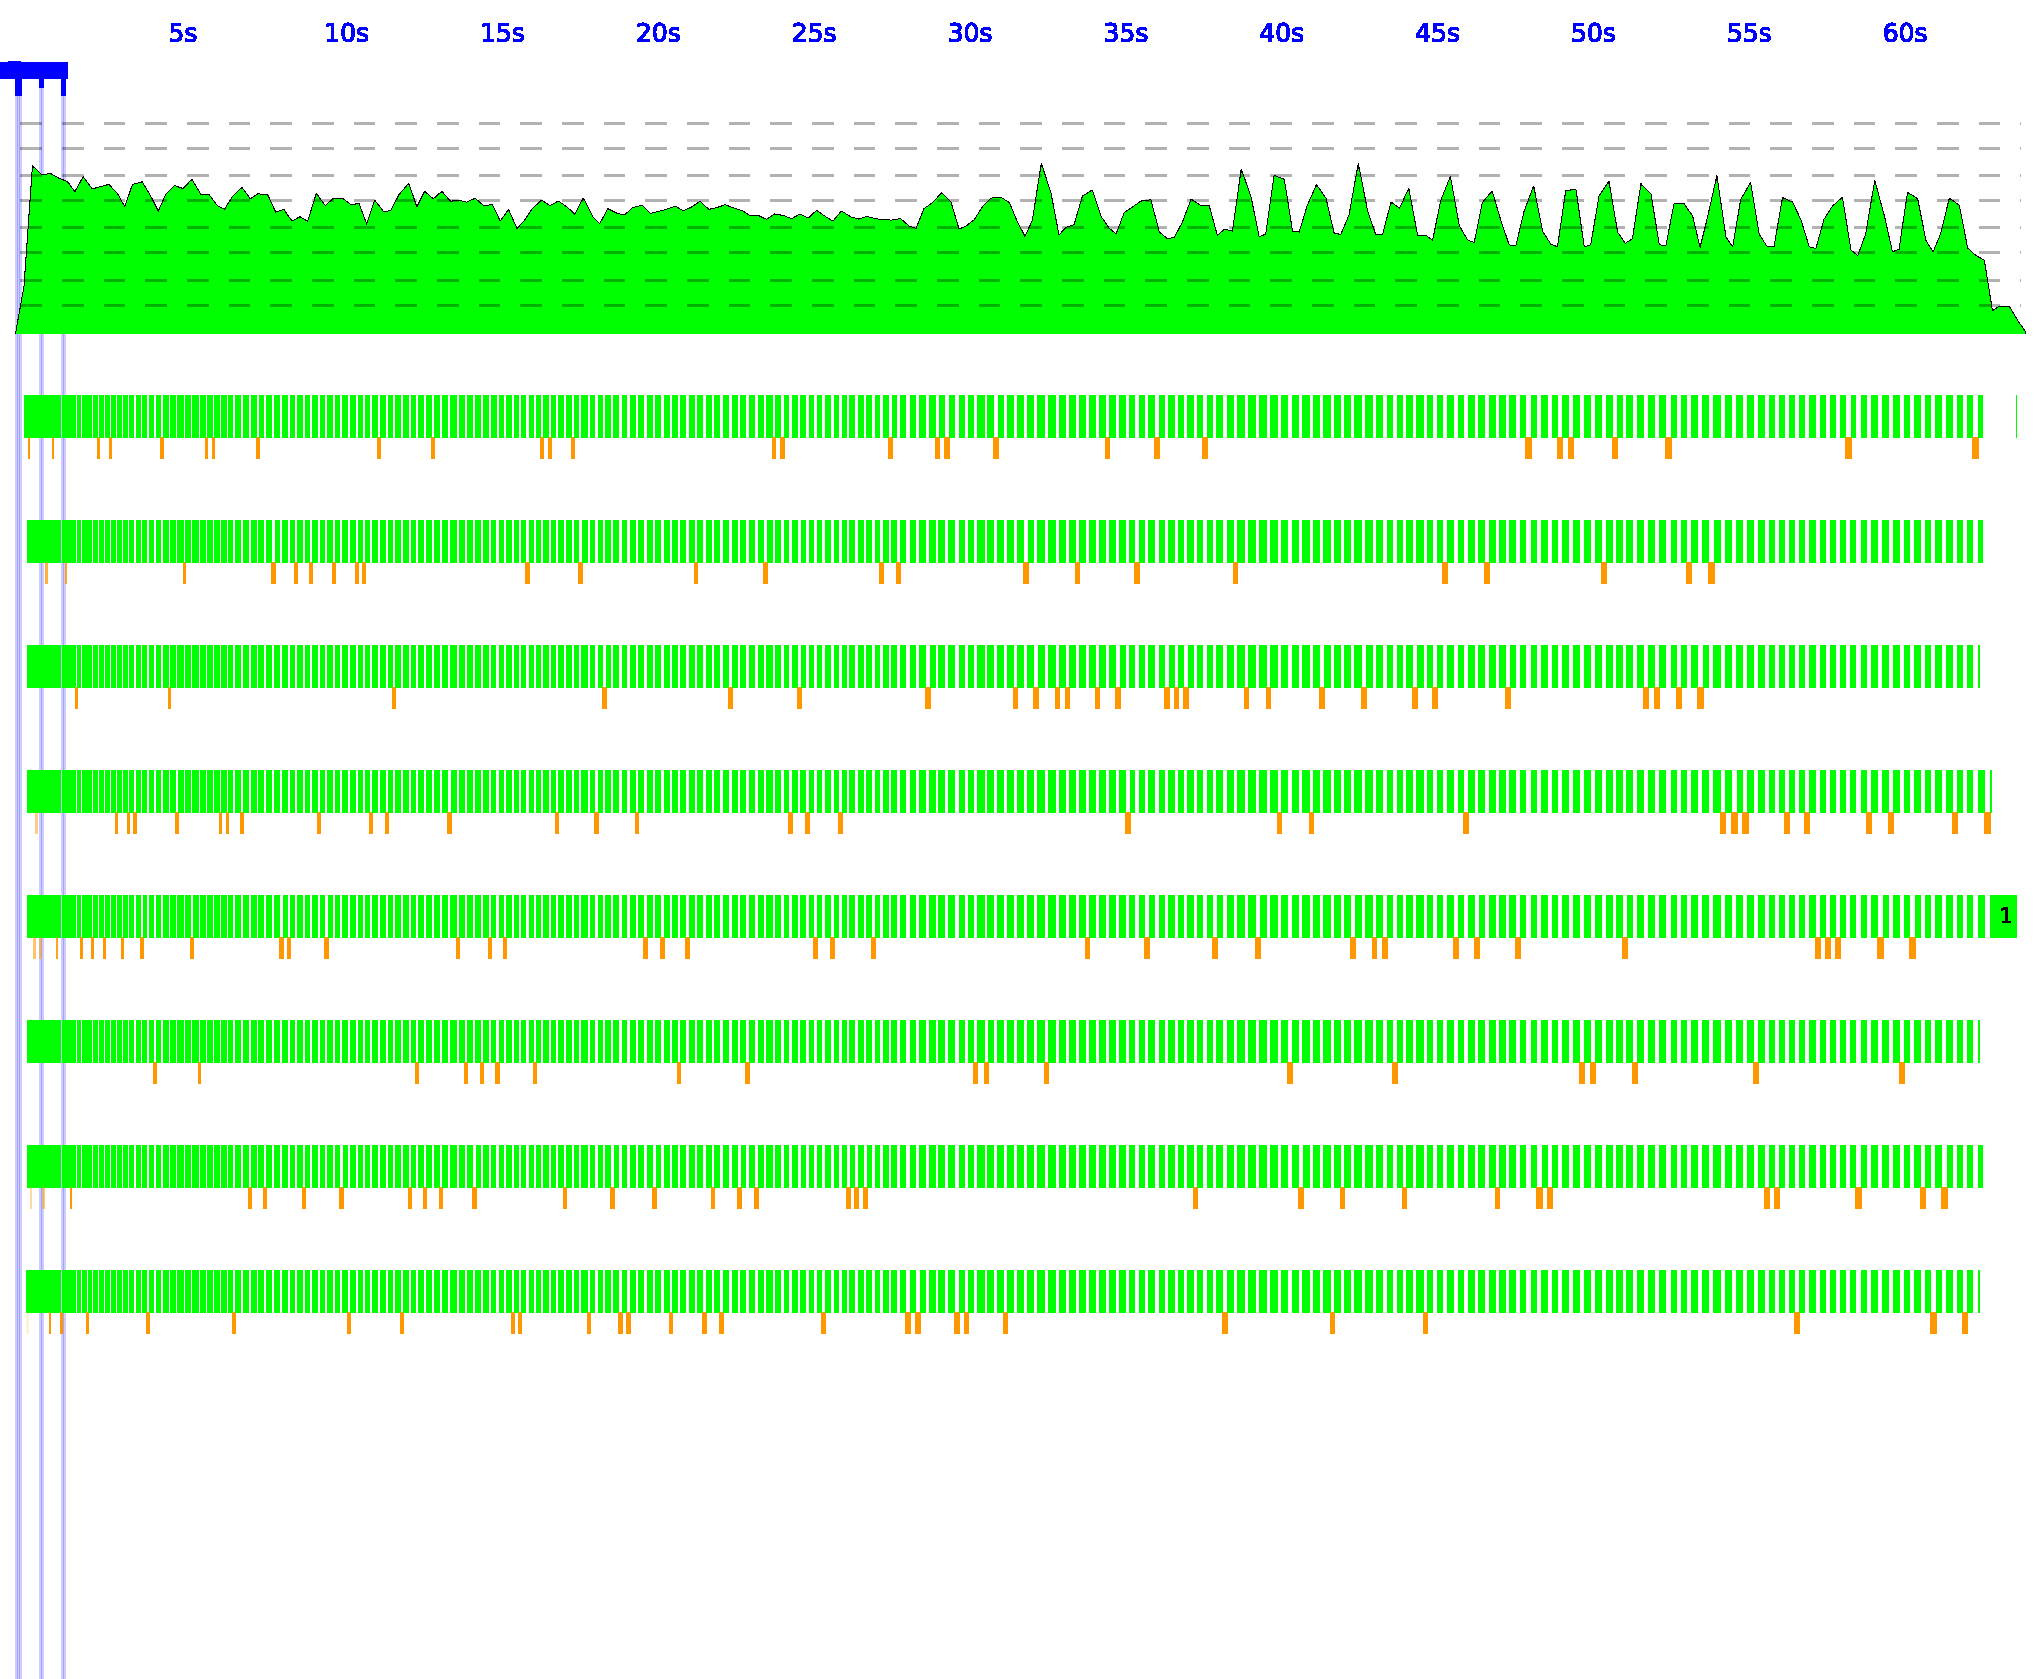
\includegraphics[width=0.98\textwidth]{pics/icfp2000_eventlog}
\caption{A profile of the raytracer}
\label{fig:ts_icfp2000}
\end{figure}

Some of our early examples use only the \tscope features introduced by the
GHC developers.
We modified Mercury's runtime system to write out compatible log files using
only the events in Section~\ref{sec:tscope_background}.
Using some of the example programs from previous chapters we were able to
see the \tscope profiles of the raytracer
(Figure~\ref{fig:ts_icfp2000})
and the mandelbrot image generator (Figure~\ref{fig:ts_mandelbrot}).
These profiles were generated on an eight processor machine, using eight
Mercury engines.
In both figures, green areas in the eight lower rows indicate when each of
the eight Mercury engines was executing a context.
Orange areas indicate when that engine initiated garbage collection.
The top-most row shows, at each point in time, how many engines are
executing contexts.

In Figure~\ref{fig:ts_icfp2000} we can see the effect on runtime of the
garbage collector (GC).
The mutator is interrupted many times for short periods of time while the
GC runs.
This profile was generated with the default initial heap size,
therefore GC events occur quite frequently.

\begin{figure}
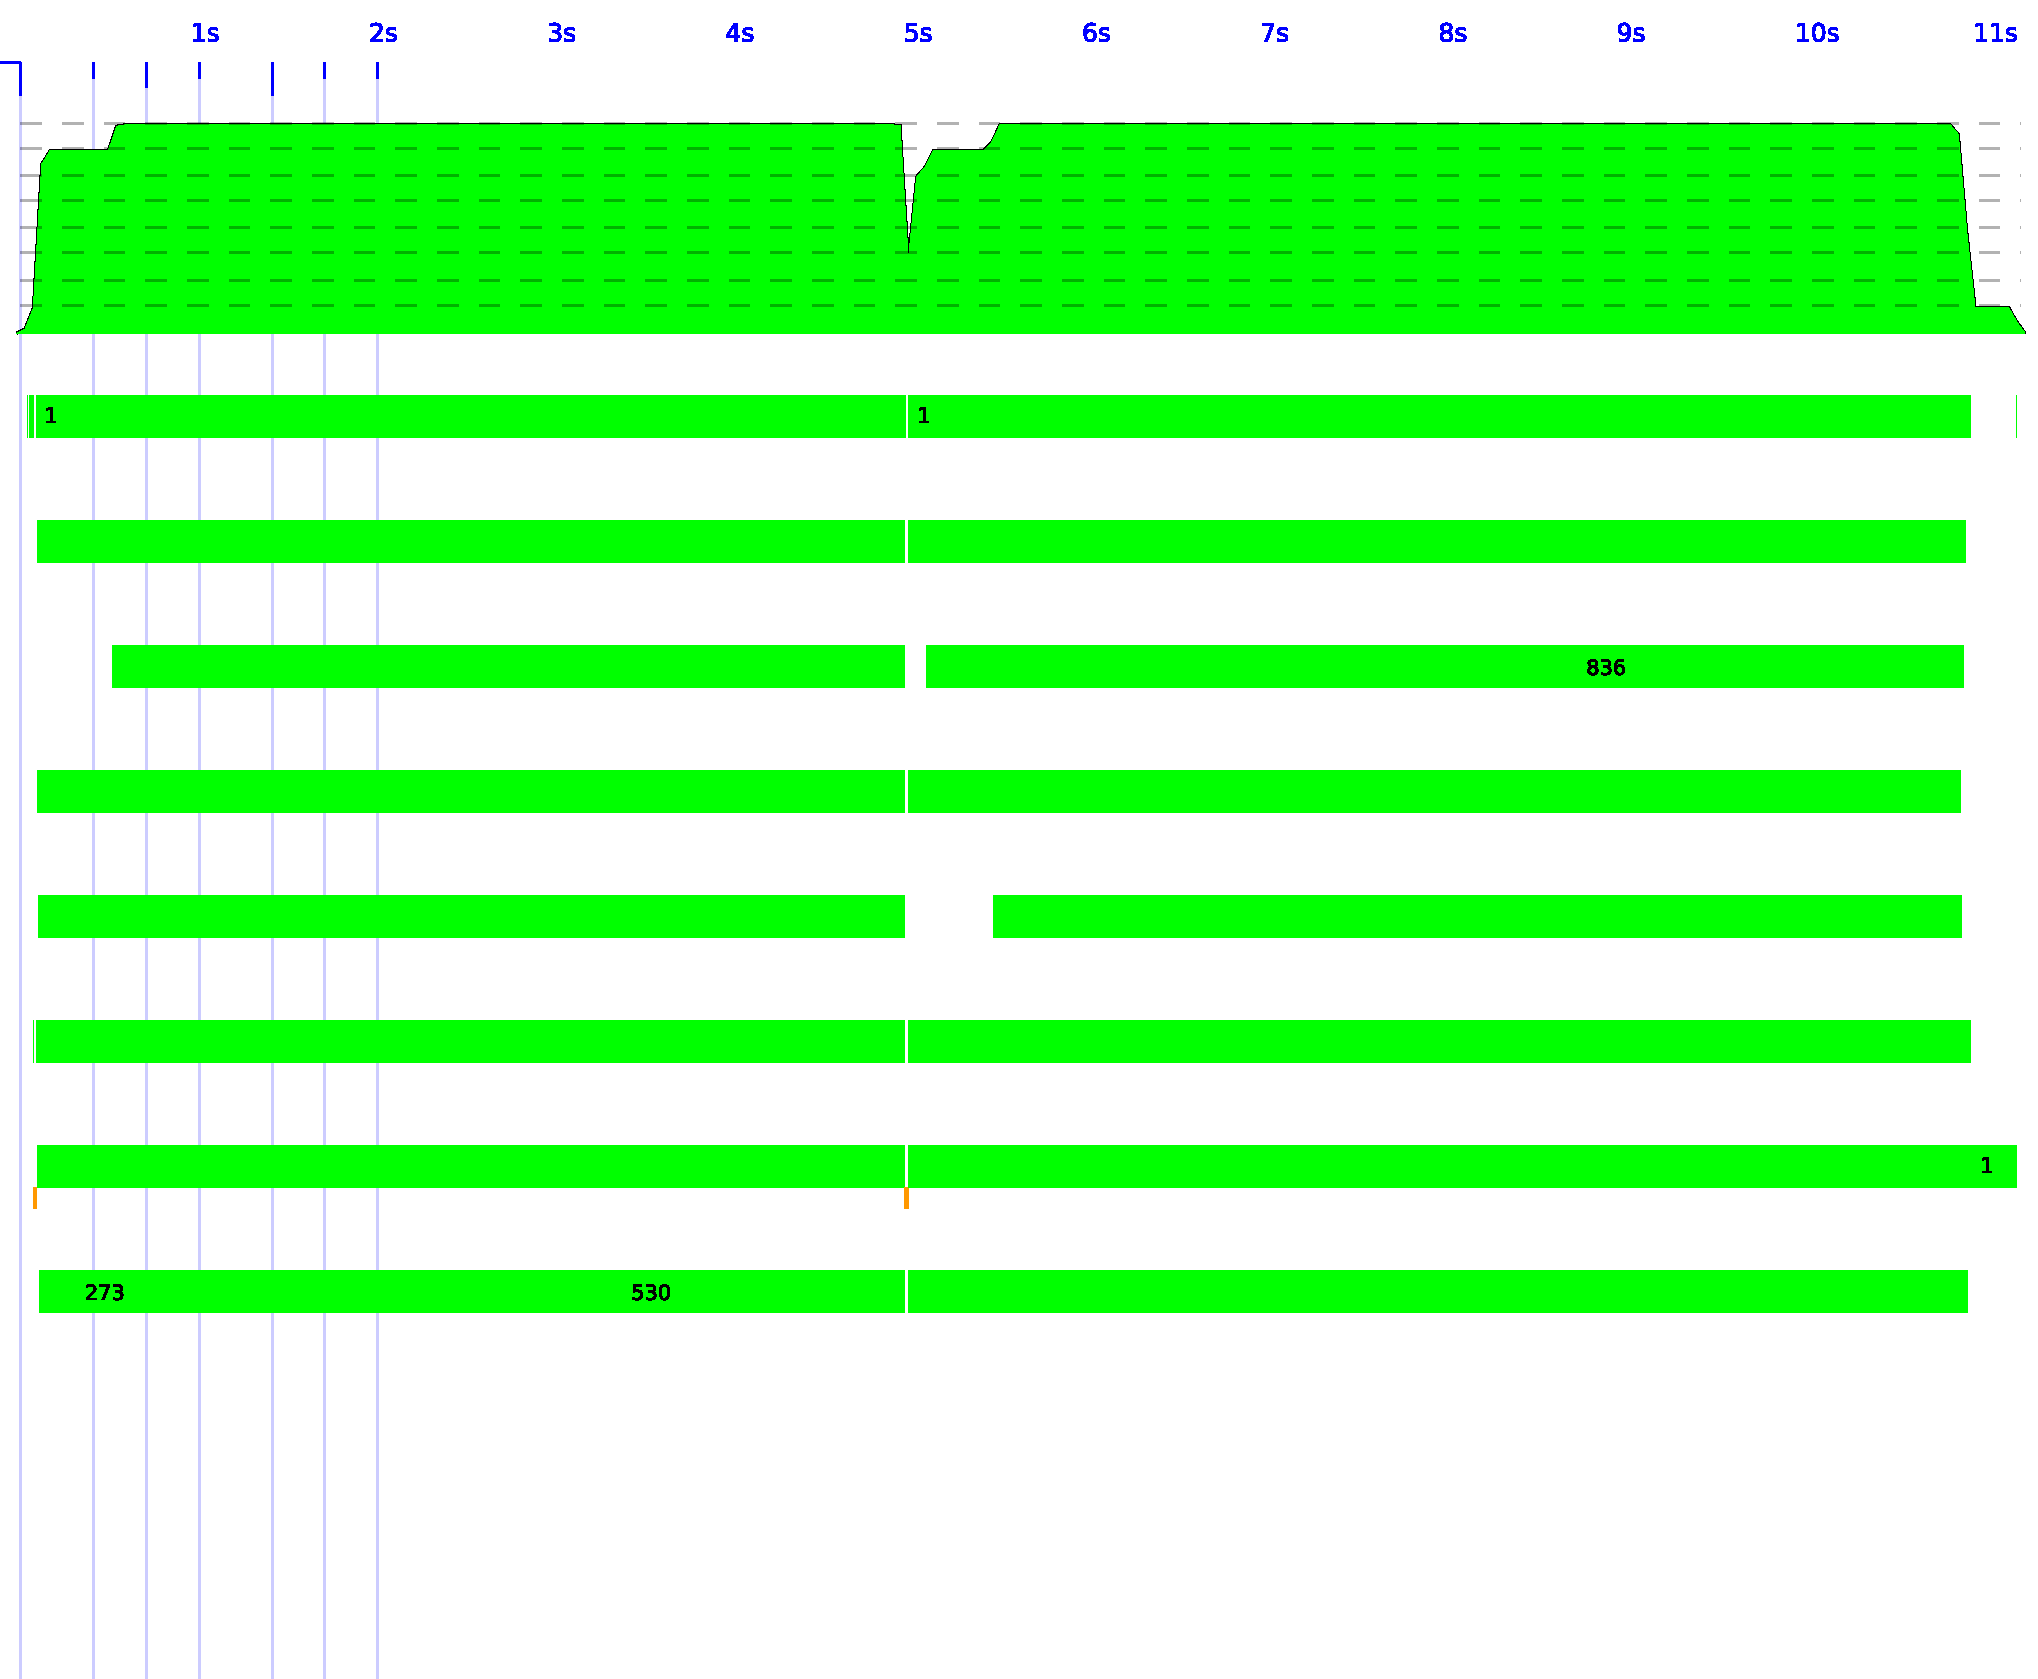
\includegraphics[width=0.98\textwidth]{pics/mandelbrot_eventlog}
\caption{A profile of the mandelbrot program}
\label{fig:ts_mandelbrot}
\end{figure}

The profile in Figure~\ref{fig:ts_mandelbrot} has a much lower memory
allocation rate.
One collection event can be seen roughly in the middle of execution,
and there is another one that cannot be seen at the beginning of the
execution\footnote{
    The \tscope tool allows us to zoom into executions,
    and small events such as very short garbage collections can be seen with
    higher magnification.}.
After the visible GC event,
we can see that the third and fifth engines do not resume their work
immediately;
this is a potential area of optimisation that runtime system programmers
could improve.

In Section~\ref{sec:rts_gc} we spoke about the impact of garbage collection
in detail.
The data for Table~\ref{tab:gc_amdahl} in that section was collected using
\tscope.
In particular we used the \metric{GC stats} and \metric{Mutator vs GC time}
metrics.
Figure~\ref{fig:ts_dat} shows this data for the
raytracer using initial heap sizes of 16MB and 512MB.
They report data averaged over eight executions,
as our command line tool supports merging \tscope reports.
We can see that the number of collections, 
the average time of a collection,
and the total time spent performing collection vary dramatically.
Which we explored in detail in Section~\ref{sec:rts_gc}.

\begin{figure}
\begin{center}
\begin{minipage}[b]{0.49\textwidth}
\subfigure[16MB initial heap size] \\
\code{~~~~Running time:~~~~~~~13.45s~~~100.0\%} \\
\code{~~~~Number of collections:~288} \\
\code{~~~~Total GC time:~~~~~~~~~7.05s~~~52.4\%} \\
\code{~~~~Total Mut time:~~~~~~~~6.40s~~~47.6\%} \\
\code{~~~~Average GC time:~~~~~~~24.48ms} \\
\end{tabular}
}}
\end{minipage}
%
\begin{minipage}[b]{0.49\textwidth}
\subfigure[512MB initial heap size] \\
\code{~~~~Running~time:~~~~~~~6.95s~~~100.0\%} \\
\code{~~~~Number~of~collections:~26} \\
\code{~~~~Total~GC~time:~~~~~~~~~1.25s~~~17.9\%} \\
\code{~~~~Total~Mut~time:~~~~~~~~5.71s~~~82.1\%} \\
\code{~~~~Average~GC~time:~~~~~~~47.96ms} \\
\end{tabular}
}}
\end{minipage}
\end{center}
\caption{Basic metrics for the raytracer}
\label{fig:ts_dat}
\end{figure}

We have not yet implemented any more advanced metrics.
However, even our simplest metrics have already been useful.

\section{Related work and conclusion}
\label{sec:tscope_conc}

% It is well established that a visualisation tool is extremely useful
% for programmers debugging and tuning complex systems.
% \tscope definitely supports this when used either with
% Haskell \citep{threadscope},
% or, as we have proposed, when used with Mercury.
% Furthermore, extending \tscope to work with Mercury has been
% relatively straight forward,
% largely due to \tscope's extensible file format.
%
% Other tools have existed for profiling the parallel execution of other
% languages such as Eden's trace viewer \citep{edentraceviewer}.
% This shows a similar timeline to that of threadscope,
% but since Eden is a distributed programming language it also shows
% communication.
%
% GranSim \citep{loidl98:gransim} is a simulator that determines how much
% parallelism is in a Haskell program.
% Ben Lippmeier wrote a similar tool/paper, its on his website.
%
% \citet{runciman93:profilingparfp} introduces another visualisation tool.
% This also shows the amount of parallelism in a Haskell program, but it does it
% over time and also shows the number of blocked tasks.
%
% Apparently GUM has some good profiling tools, but I did not read this
% paper \citep{trinder:1996:gum}

% Use this as a source of feedback.
% Discuss what this work implies for Haskell.
% Discuss how this can possibly be tied to perf(1).

Many parallel implementations of programming languages
come with visualisation tools
since (as we argued in the introduction)
the people writing parallel programs
need such tools to understand the actual behaviour of their programs,
and the people implementing those languages find them useful too.
Such tools have been created for all kinds of programming languages:
imperative (even Visual Studio has one),
functional
(\citet{edentraceviewer,loidl98:gransim,runciman93:profilingparfp} among others)
and logic (\citet{Foster96,vace}
and the systems cited by \citet{Gupta95parallelexecution}).

Many of these visualisers share common ideas and features.
For example, many systems (including \tscope)
use a horizontal bar with different parts coloured differently
to display the behaviour of one CPU,
while many other systems use trees
that display the structure of the computation.
(The latter approach is more common
among visualisers for sequential languages.)
Nevertheless, each visualiser is necessarily oriented
towards giving its users what they want,
and the users of different systems want different information,
since they are using different languages based on different concepts.
For example, functional languages have no concept of parallel conjunctions,
and their concept of data flow between computations
is quite different from Mercury's,
and users of concurrent logic programming languages
such as Concurrent Prolog, Parlog and Guarded Horn Clauses
have quite different concerns from users of Mercury
(where to disable parallelism, not where to enable it).

We know of only one visualiser
for a not-inherently-concurrent logic programming language
that does nevertheless support dependent AND-parallelism: VACE \citep{vace}.
However, the ACE system supports
OR-parallelism and independent AND-parallelism
as well as dependent AND-parallelism,
and its features do not seem designed
to help programmers exploit dependent AND-parallelism better.
As far as we know, no-one has built a profiler
for a dependent AND-parallel logic programming language
with the capabilities that we propose.
We haven't yet built one either,
but we are working on it.
% We expect to have at least a third of our proposed metrics implemented
% by the time of the workshop,
% and many more by the end of the year.

% I think our basic argument should be:
% - visualisation tools have long proven to be useful
%   in improving the performance of parallel programs
%   and in helping the developers of parallel systems
% - such tools have been built for many different systems:
%   logic, functional, and imperative,
% - some features are common to many of these systems:
%   many show trees, while many others show CPU utilization
% - yet each visualiser is nevertheless specific to its own language
% - the only visualiser (VACE) we know of for a language
%   that supports dependent AND parallelism
%   does not focus on dependent AND parallelism,
%   and it does not gather the metrics we think we need

% You can find these papers in ~pbone/papers/
% berthold_eden.pdf
% runciman_Profiling-par-fp.pdf
% I did not download the gransim or gum papers.

% zs: the relevant papers I found are in the files
% vace.ps
% hotpar10.pdf
% par_prolog_survey.pdf
% CRPC-TR93446.pdf
% in my home directory.

